\chapter{Kết luận và Hướng phát triển}
\label{chap:conclusion}

Đồ án đã bước đầu hoàn thành giai đoạn thiết kế và kiểm chứng mô hình 
cho một hệ thống Edge AI hiệu năng cao trên nền tảng FPGA. 
Chương này tổng kết các kết quả đạt được, nghiên cứ phần hiện thực kỹ thuật 
và đề ra lộ trình chi tiết cho giai đoạn hiện thực phần cứng.

\section{Kết quả đạt được}
Trong giai đoạn này, đồ án đã hoàn thành thiết kế kiến trúc hệ thống và 
chuẩn bị tài nguyên phần mềm, cụ thể:

\begin{enumerate}
    \item \textbf{Đề xuất kiến trúc SoC dị thể tối ưu:} Đã thiết kế chi tiết hệ thống tích hợp giữa Vi xử lý ứng dụng (ARM Cortex-A53 trên Zynq UltraScale+), Vi xử lý điều khiển lõi mềm (RISC-V PULP) và Khối tăng tốc phần cứng (CNN Accelerator). Kiến trúc này giải quyết bài toán cân bằng giữa tính linh hoạt và hiệu năng tính toán.
    
    \item \textbf{Thiết kế chi tiết các phân hệ giao tiếp:}
    \begin{itemize}
        \item Quy hoạch thành công bản đồ bộ nhớ (Memory Map) cho hệ thống chia sẻ tài nguyên.
        \item Thiết kế cơ chế giao tiếp liên nhân (Inter-core Communication) sử dụng Mailbox và giao thức bắt tay (Handshaking) để đồng bộ hóa dữ liệu giữa miền PS (Linux) và PL (Bare-metal).
        \item Xây dựng sơ đồ luồng dữ liệu (Dataflow) tối ưu hóa cho truy cập bộ nhớ dạng Burst qua AXI4.
    \end{itemize}

    \item \textbf{Xây dựng và Tối ưu hóa Mô hình AI:}
    \begin{itemize}
        \item Lựa chọn và huấn luyện thành công mạng MobileNetV1 cho bài toán phát hiện người (Human Detection) với độ chính xác khả quan trên tập kiểm thử.
        \item Hoàn tất quy trình Lượng tử hóa (Quantization) từ Float32 sang Int8, giúp giảm 4 lần kích thước mô hình mà không làm giảm đáng kể độ chính xác.
        \item Chuyển đổi thành công mô hình sang định dạng mảng C (Header files), sẵn sàng cho việc nhúng xuống phần cứng.
    \end{itemize}
\end{enumerate}

\section{Khó khăn và Hạn chế}
Trong quá trình thực hiện, nhóm đã gặp phải và xử lý một số thách thức kỹ thuật:

\begin{itemize}
    \item \textbf{Sự phức tạp của giao tiếp AXI:} Việc đồng bộ hóa giữa miền xung nhịp cao (1.2 GHz của ARM) và miền xung nhịp thấp (100 MHz của FPGA) đòi hỏi thiết kế bộ đệm và cơ chế CDC (Clock Domain Crossing) cẩn trọng để tránh mất mát dữ liệu.
    \item \textbf{Thiên kiến dữ liệu (Data Bias):} Các bộ dữ liệu ban đầu (ảnh chân dung/khuôn mặt) không phù hợp với góc nhìn thực tế của Camera giám sát. Vấn đề này đã được khắc phục bằng việc chuyển sang sử dụng bộ dữ liệu chuẩn hóa (như INRIA Person Dataset/COCO) chứa ảnh toàn thân và bối cảnh đa dạng.
    \item \textbf{Giới hạn bộ nhớ nội (On-chip Memory):} Dung lượng BRAM trên FPGA có hạn, đòi hỏi chiến lược quản lý bộ nhớ đệm dòng (Line Buffer) hiệu quả để tối ưu hóa việc tái sử dụng dữ liệu.
\end{itemize}

\newpage
\section{Kế hoạch thực hiện tiếp theo}
Giai đoạn tiếp theo sẽ tập trung vào việc hiện thực hóa thiết kế trên bo mạch vật lý Kria KV260. Các đầu việc chính bao gồm:

\begin{enumerate}
    \item \textbf{Hiện thực Phần cứng (Hardware Implementation):}
    \begin{itemize}
        \item Tiến hành Tổng hợp (Synthesis) và Thực thi (Implementation) thiết kế trên Vivado.
        \item Đóng gói Bitstream và xuất khẩu phần cứng (Hardware Export - XSA).
    \end{itemize}

    \item \textbf{Phát triển Firmware và Hệ điều hành:}
    \begin{itemize}
        \item Xây dựng bản dựng PetaLinux tùy biến, tích hợp driver UIO để truy cập vùng nhớ vật lý.
        \item Lập trình Firmware C cho nhân RISC-V, tích hợp các mảng trọng số đã xuất ra từ Phase 1.
    \end{itemize}

    \item \textbf{Tích hợp và Đánh giá thực nghiệm:}
    \begin{itemize}
        \item Chạy thử nghiệm hệ thống với Camera MIPI CSI-2 theo thời gian thực.
        \item Đo đạc các thông số kỹ thuật quan trọng: Tốc độ xử lý (FPS), Độ trễ (Latency) và Công suất tiêu thụ (Power Consumption).
        \item So sánh hiệu năng giữa việc chạy thuần trên ARM và chạy có tăng tốc phần cứng để minh chứng tính hiệu quả của đề tài.
    \end{itemize}
\end{enumerate}

\textbf{kế hoạch thực hiện}

\begin{figure}[!h]
    \centering
    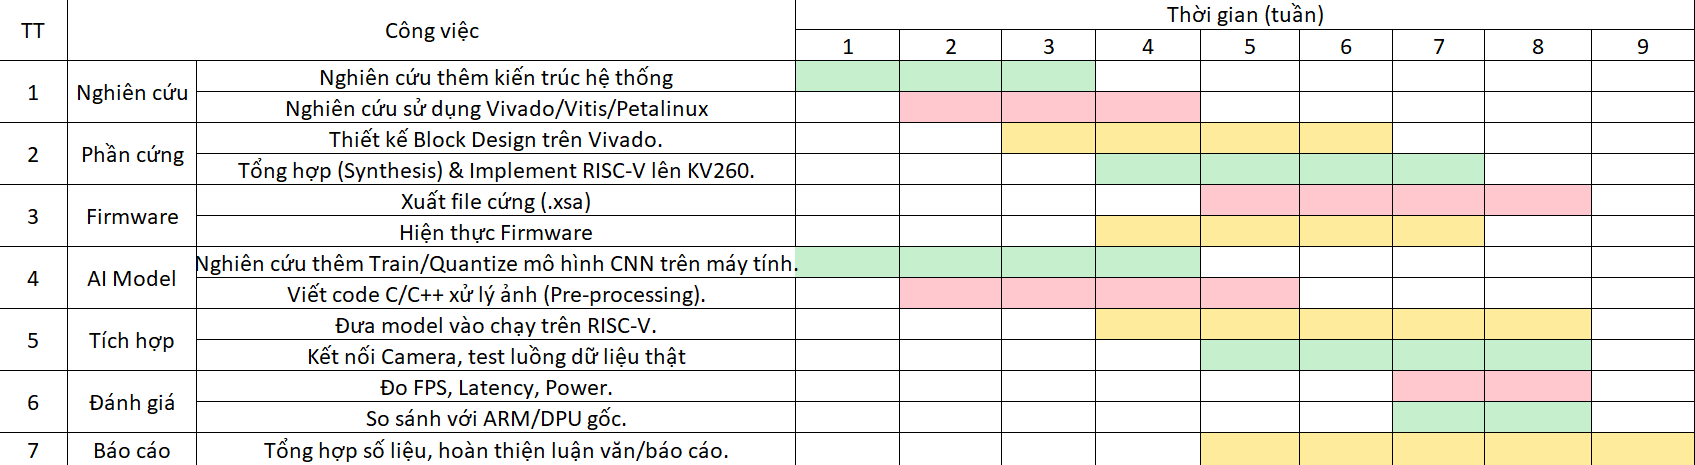
\includegraphics[width=1\textwidth]{images/conclude/gantt.png}
    \caption{Biểu đồ Gantt kế hoạch thực hiện giai đoạn hiện thực}
    \label{fig:gantt_chart}
\end{figure}